% begin module sequence-bounded-def
\begin{frame}
\begin{definition}[Bounded Sequence]
A sequence $\{ a_n\}$ is called bounded above if there exists a number $M$ such that 
\[
a_n < M \qquad \textrm{for all}\qquad  n\geq 1.
\]
It is called bounded below if there exists a number $M$ such that 
\[
a_n > M \qquad \textrm{for all}\qquad  n\geq 1.
\]
A bounded sequence is a sequence that is bounded below and above.
\end{definition}
\begin{center}
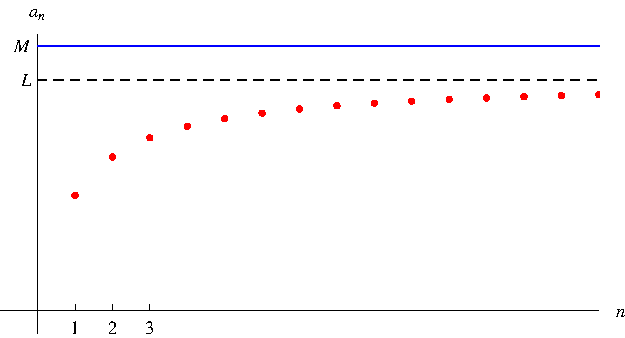
\includegraphics[height=3.5cm]{sequences/pictures/12-01-bounded.pdf}%
\end{center}
\end{frame}
% end module sequence-bounded-def
